% Page 1
\begin{figure}[H]
    \centering
    \begin{subfigure}{\textwidth}
        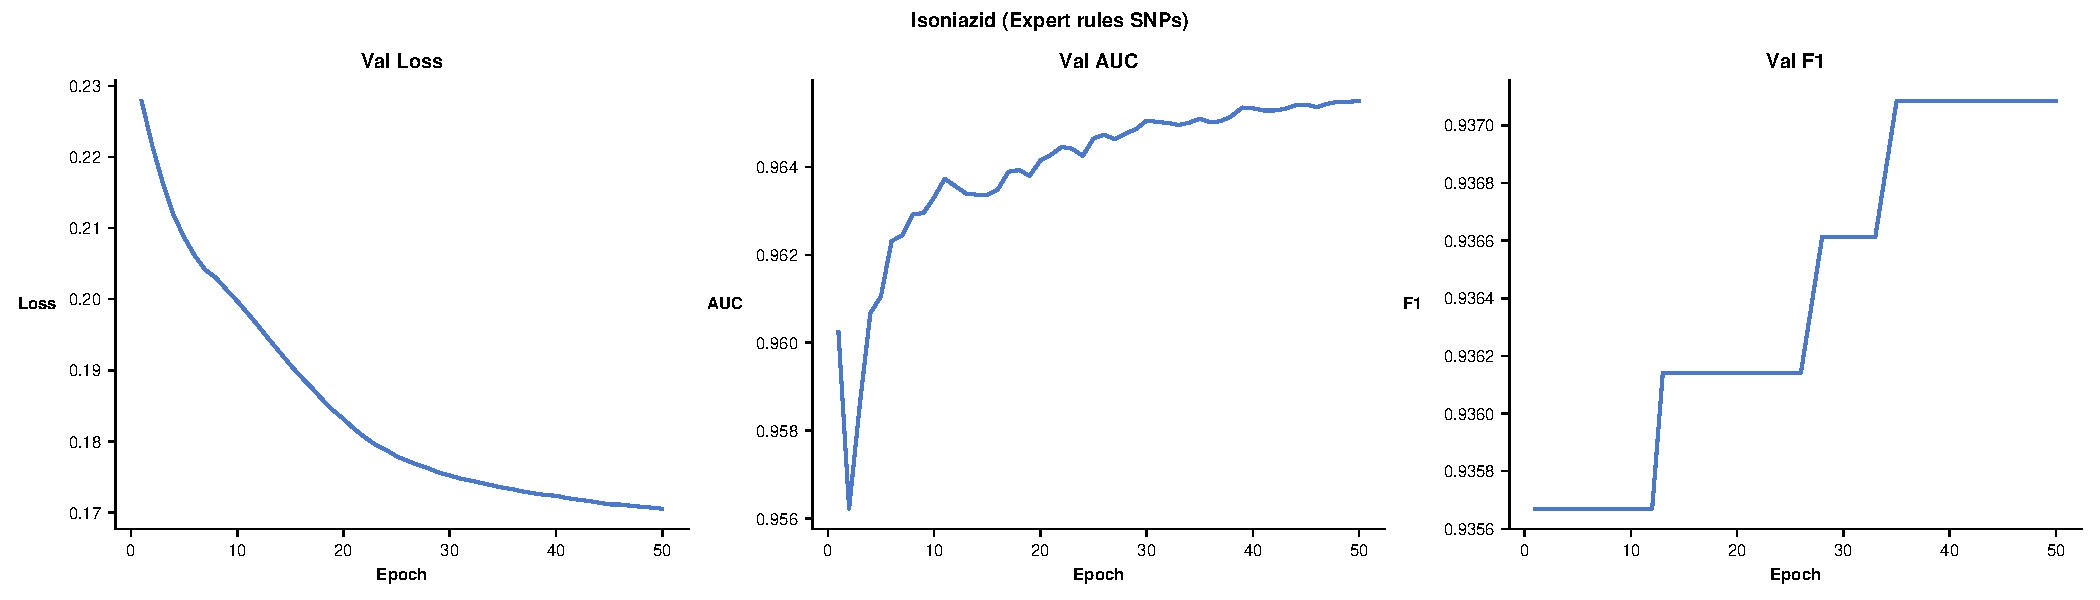
\includegraphics[width=\textwidth]{figures/expert_rules_isoniazid_learning_curves.pdf}
    \end{subfigure}
    \begin{subfigure}{\textwidth}
        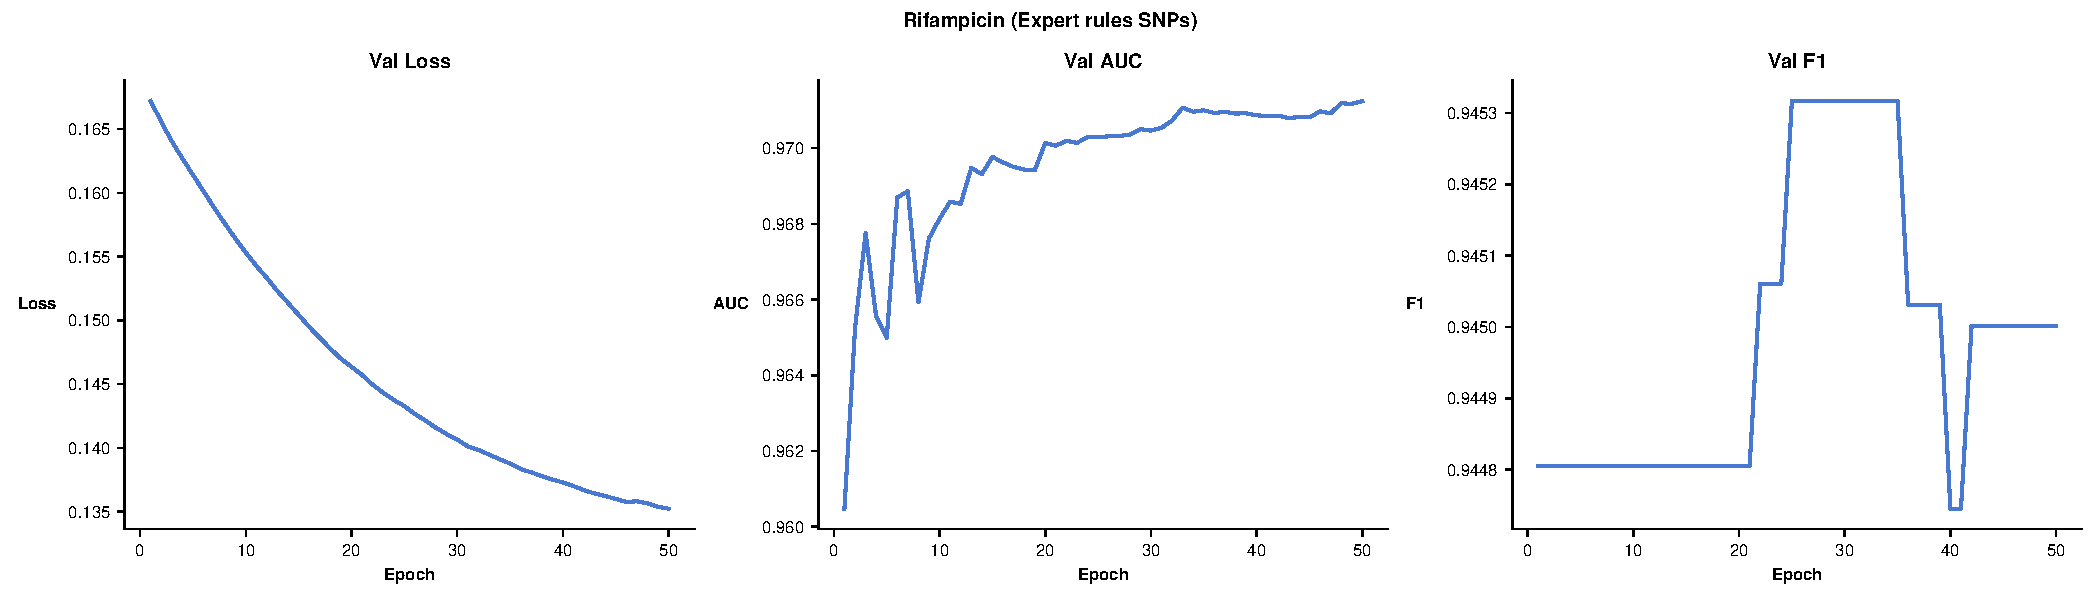
\includegraphics[width=\textwidth]{figures/expert_rules_rifampicin_learning_curves.pdf}
    \end{subfigure}
    \begin{subfigure}{\textwidth}
        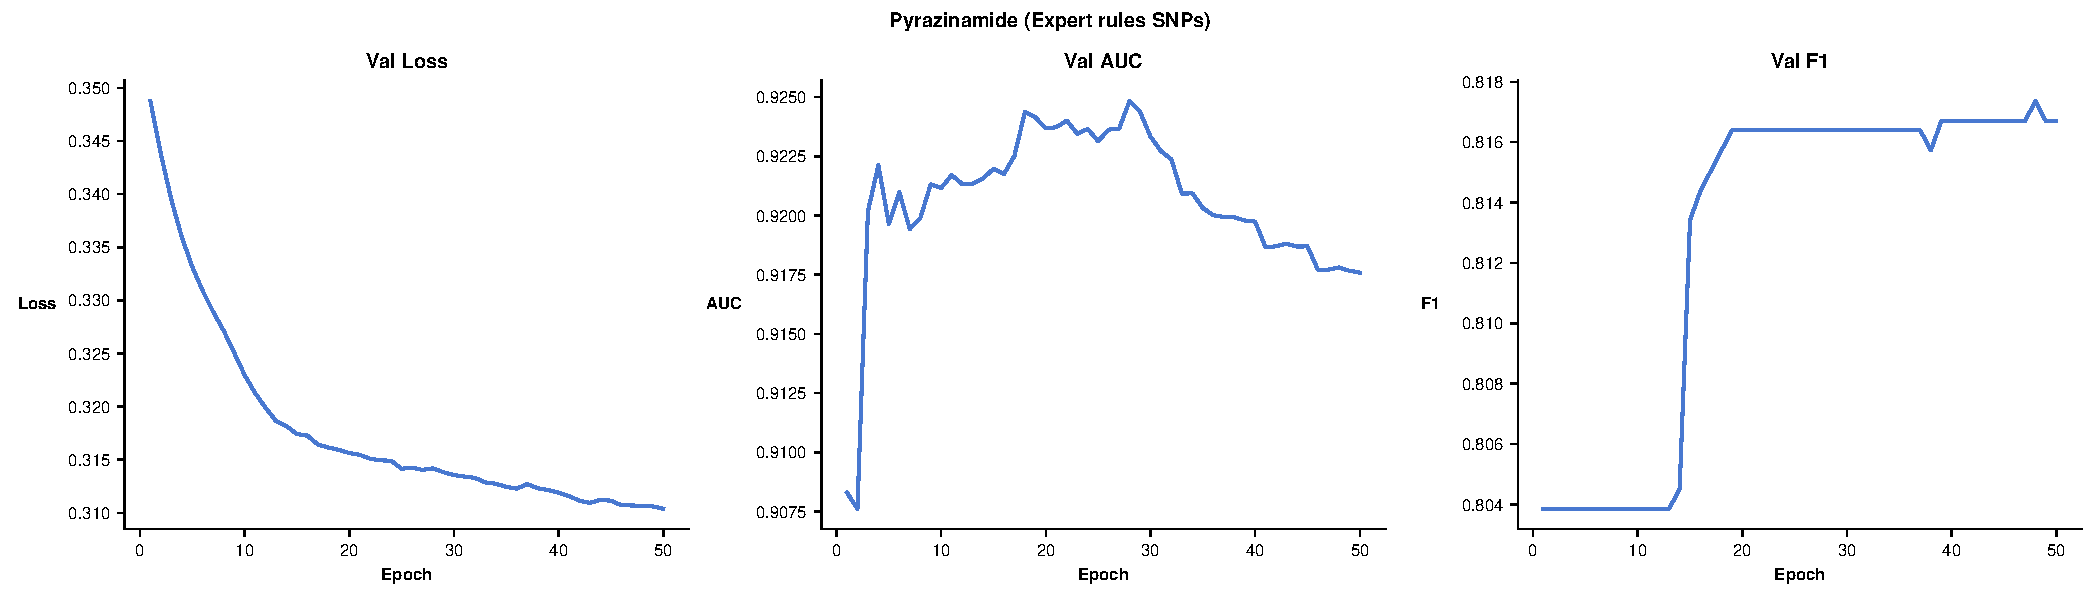
\includegraphics[width=\textwidth]{figures/expert_rules_pyrazinamide_learning_curves.pdf}
    \end{subfigure}
    \begin{subfigure}{\textwidth}
        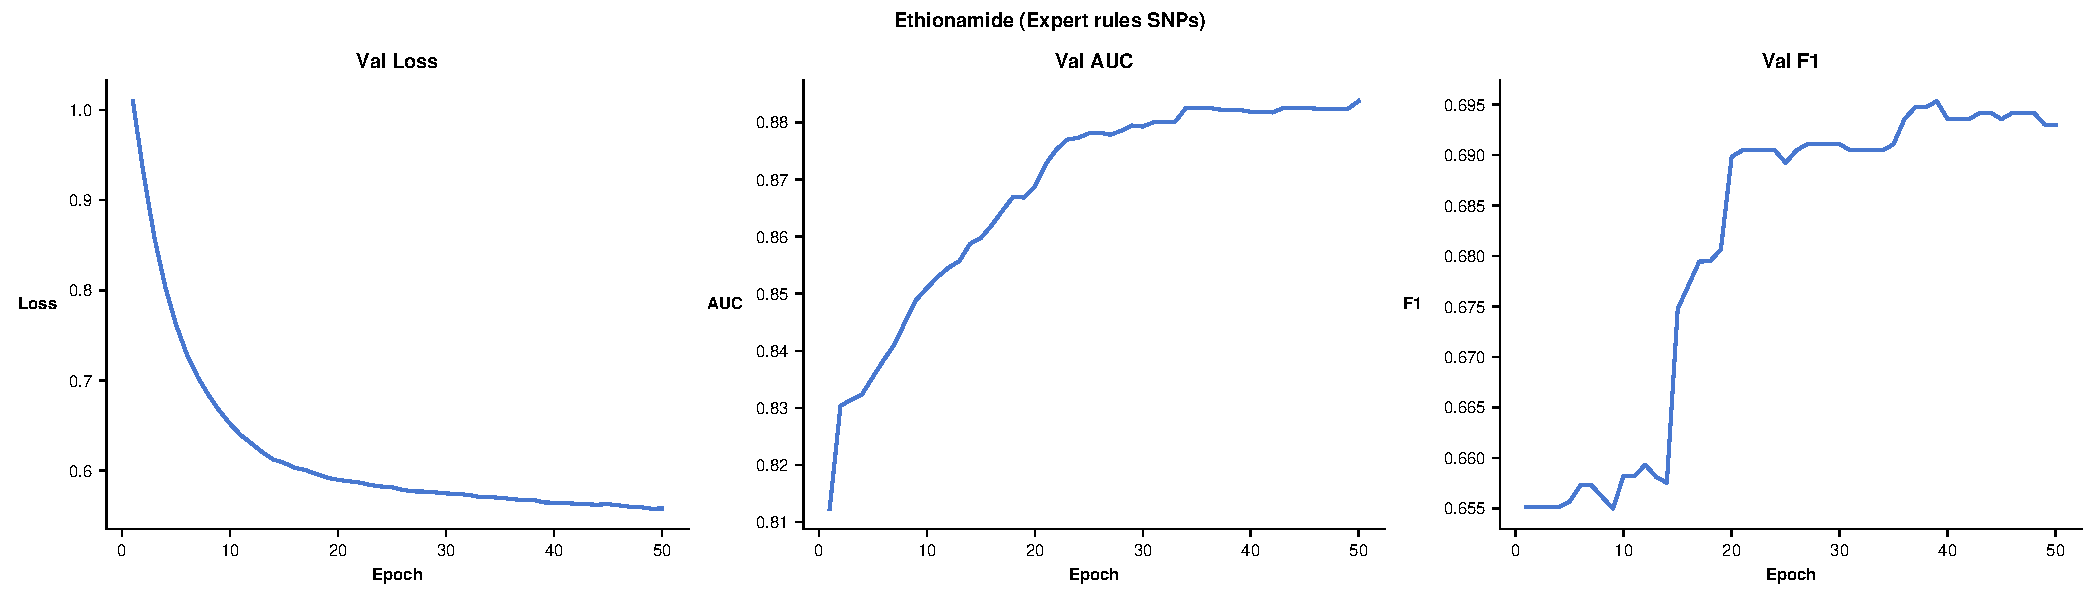
\includegraphics[width=\textwidth]{figures/expert_rules_ethionamide_learning_curves.pdf}
    \end{subfigure}
\end{figure}

\begin{figure}[H]
    \ContinuedFloat   % continues the same figure number
    \centering
    \begin{subfigure}{\textwidth}
        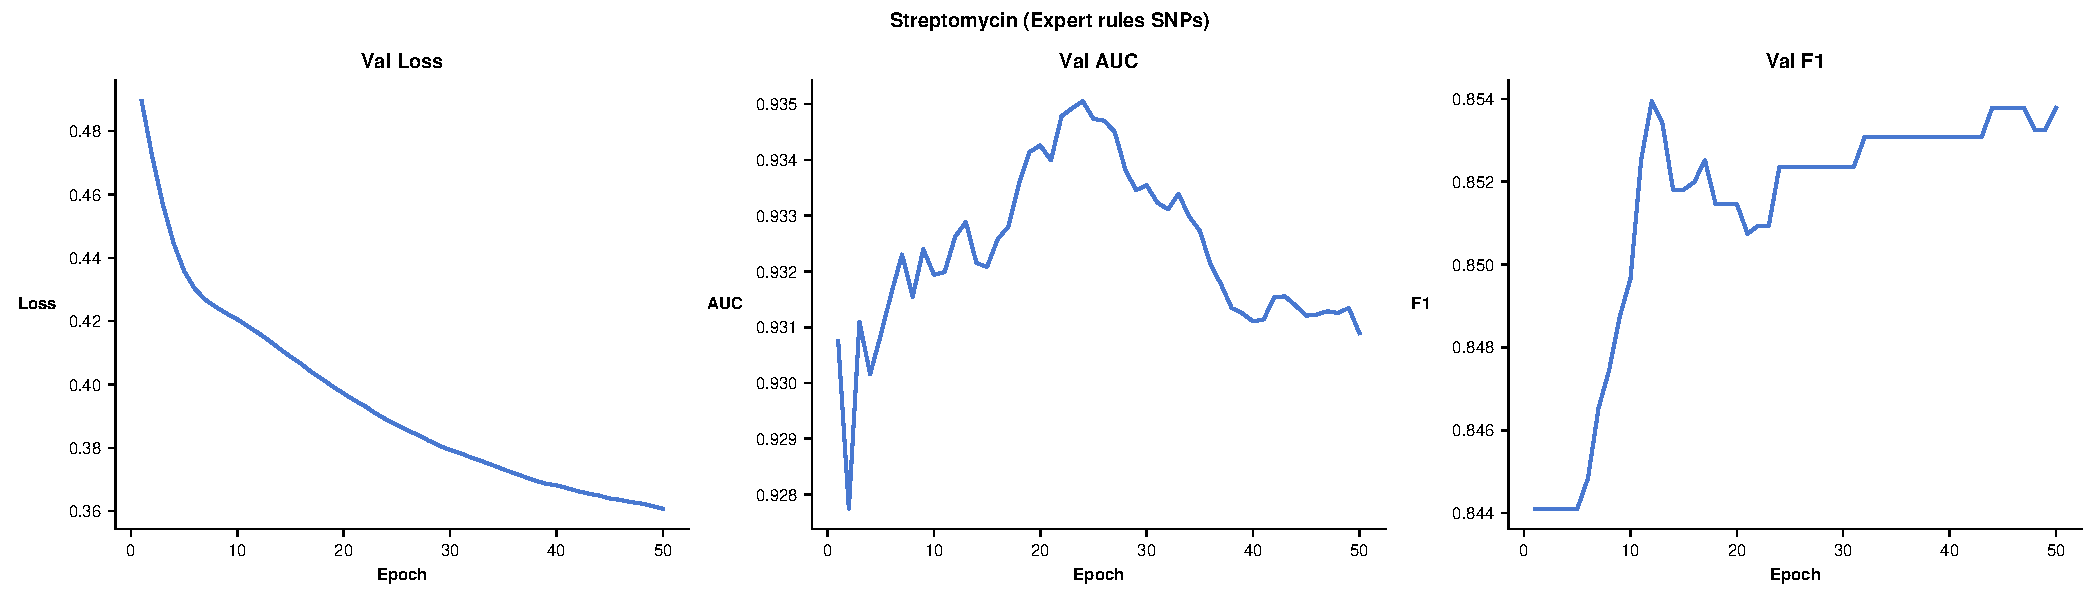
\includegraphics[width=\textwidth]{figures/expert_rules_streptomycin_learning_curves.pdf}
    \end{subfigure}
    \begin{subfigure}{\textwidth}
        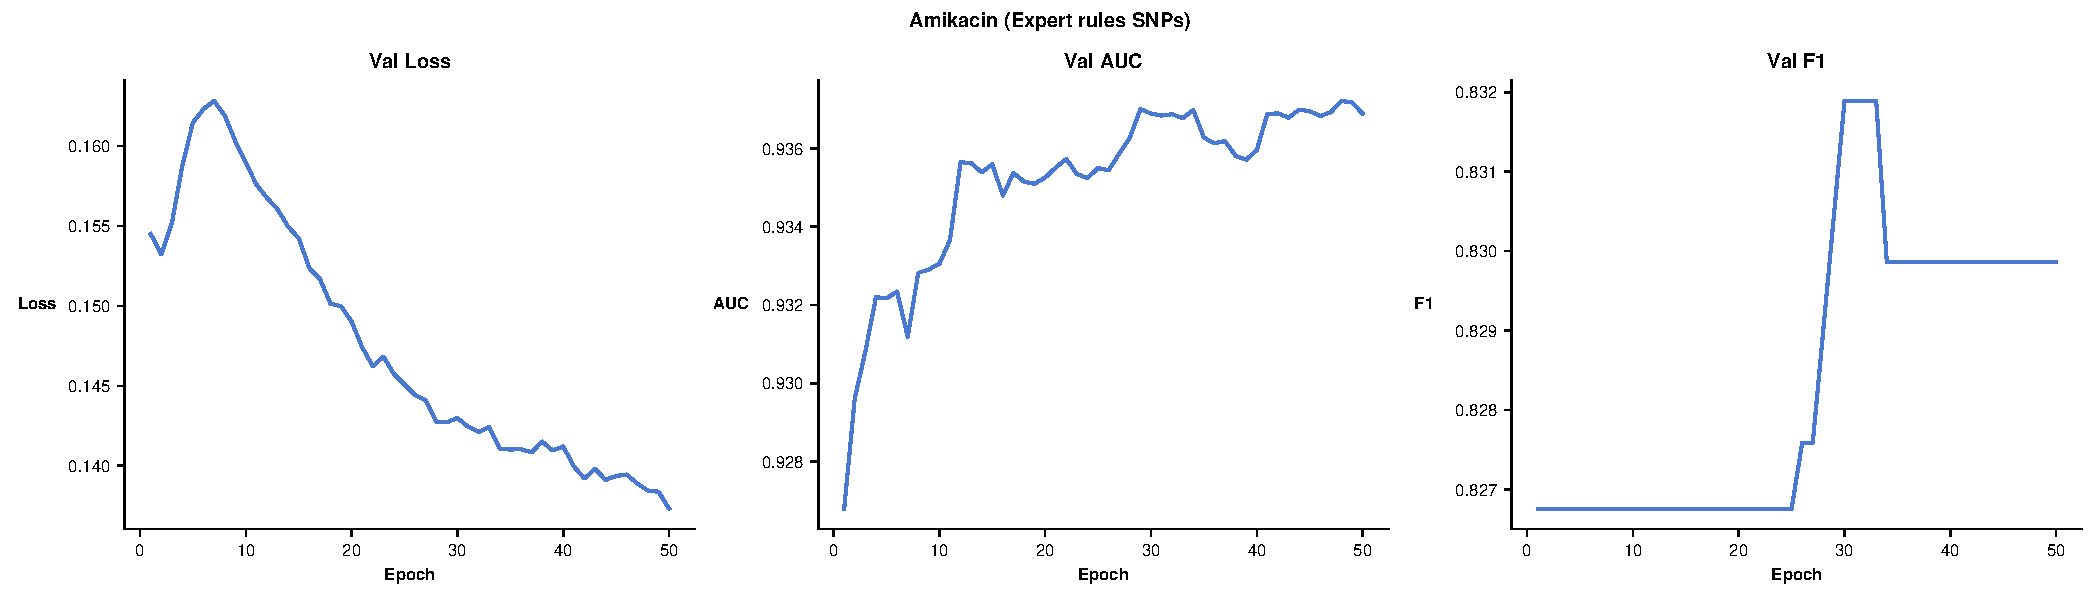
\includegraphics[width=\textwidth]{figures/expert_rules_amikacin_learning_curves.pdf}
    \end{subfigure}
    \begin{subfigure}{\textwidth}
        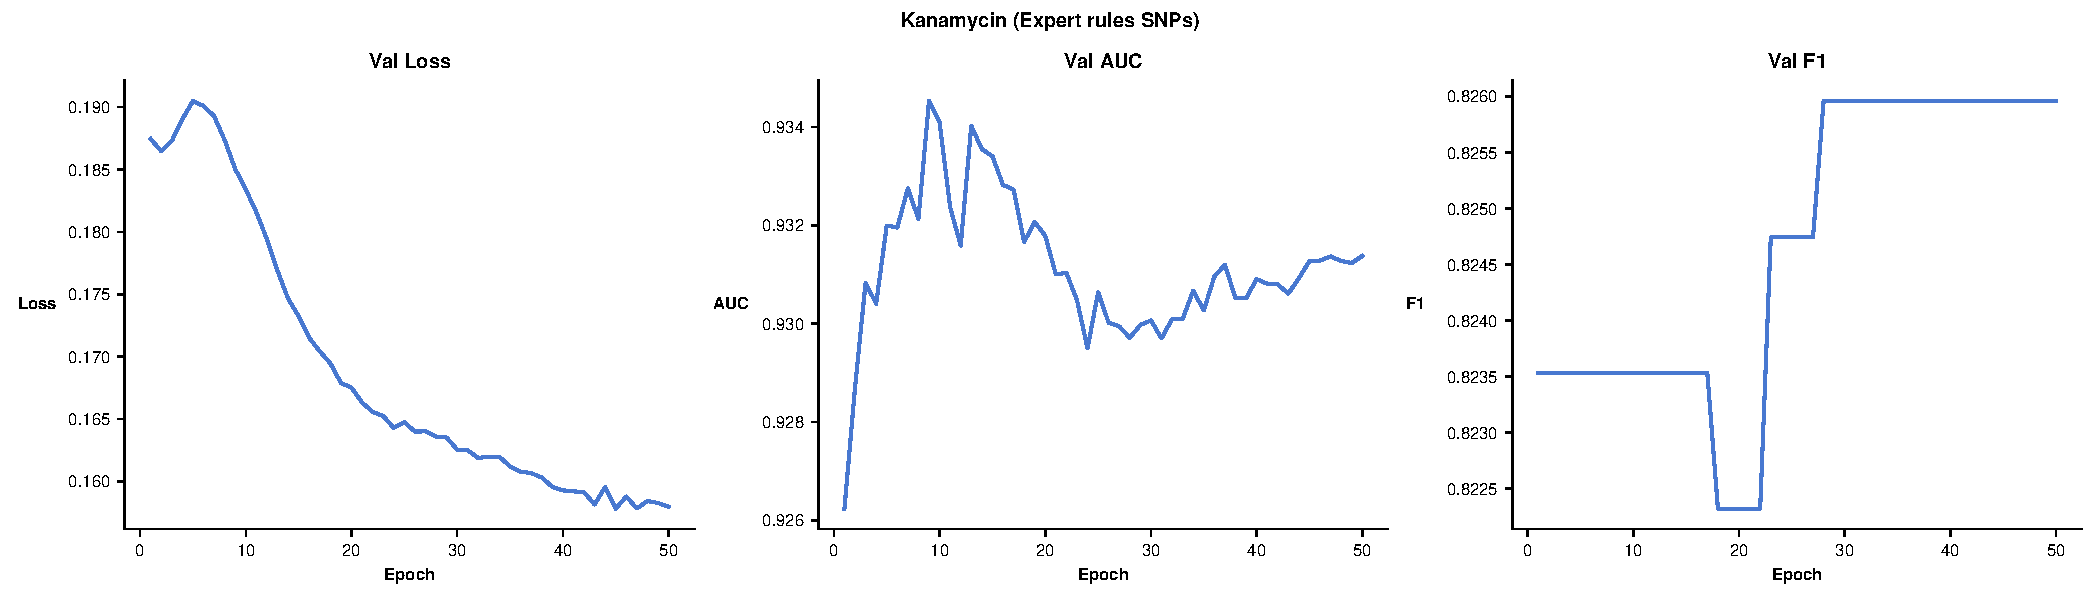
\includegraphics[width=\textwidth]{figures/expert_rules_kanamycin_learning_curves.pdf}
    \end{subfigure}
    \begin{subfigure}{\textwidth}
        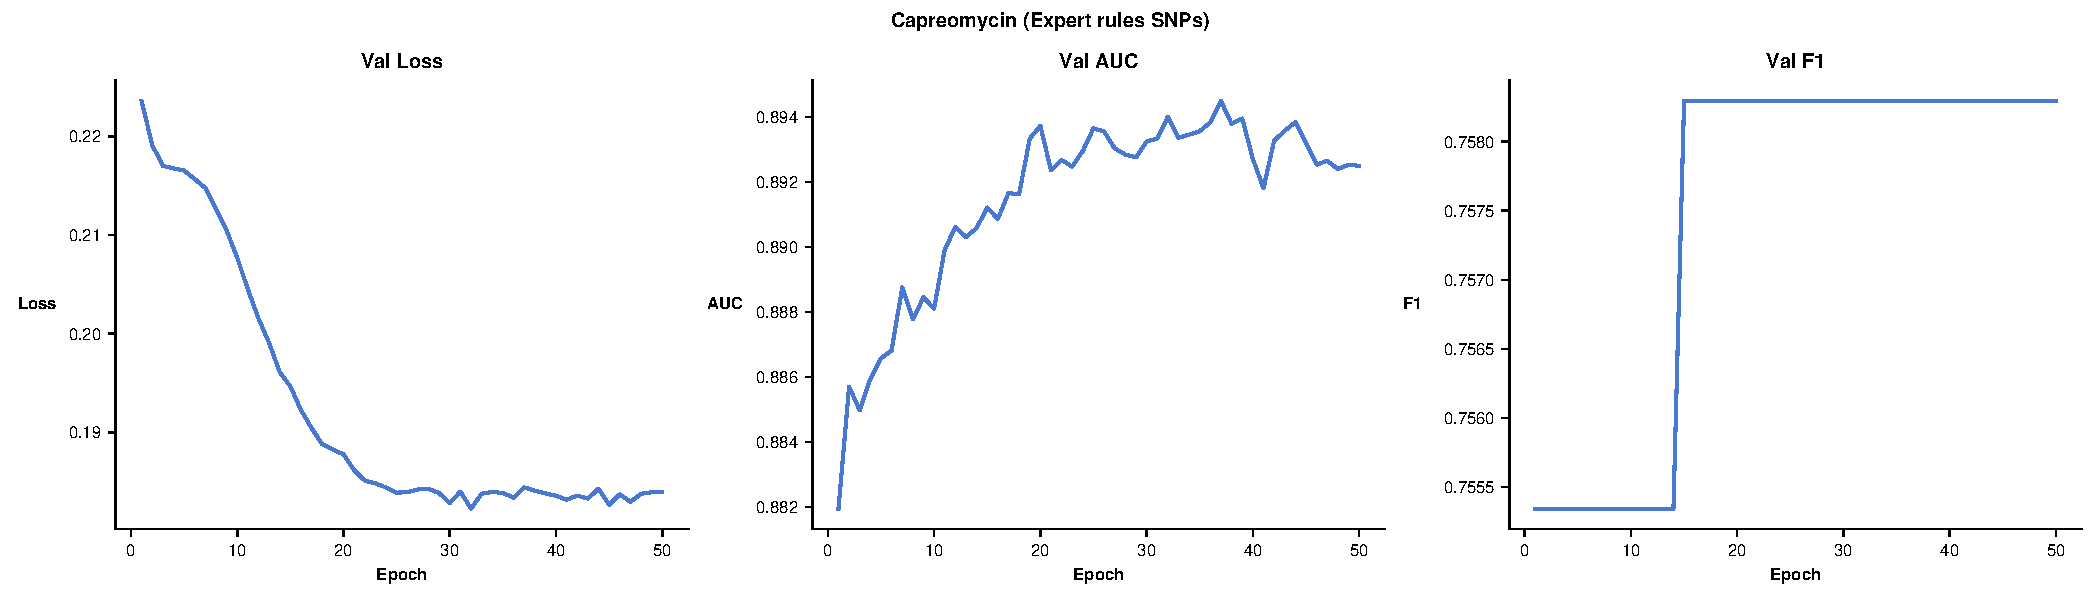
\includegraphics[width=\textwidth]{figures/expert_rules_capreomycin_learning_curves.pdf}
    \end{subfigure}
\end{figure}

\begin{figure}[H]
    \ContinuedFloat
    \centering
    \begin{subfigure}{\textwidth}
        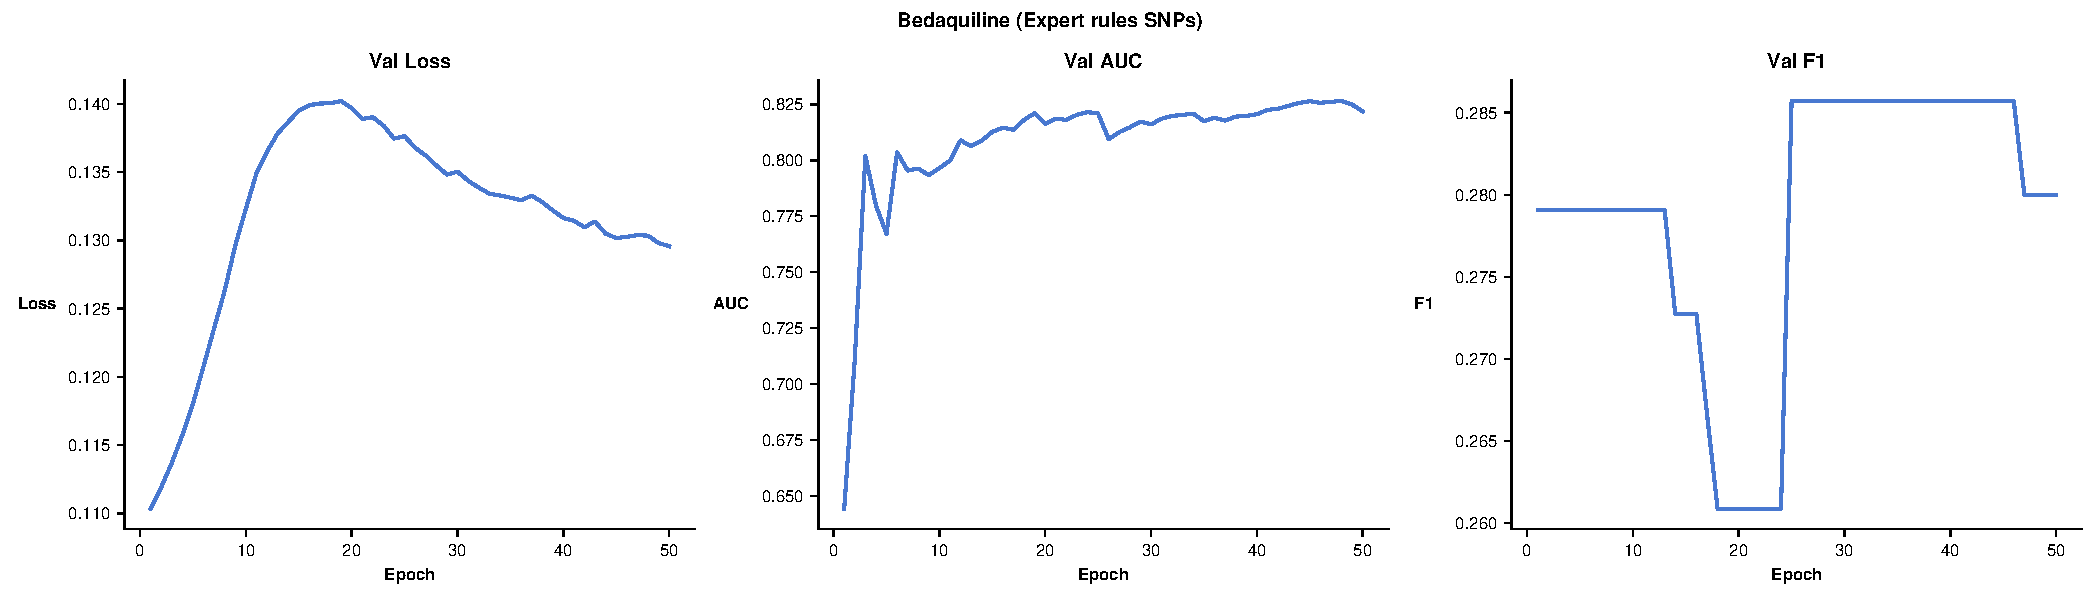
\includegraphics[width=\textwidth]{figures/expert_rules_bedaquiline_learning_curves.pdf}
    \end{subfigure}
    \begin{subfigure}{\textwidth}
        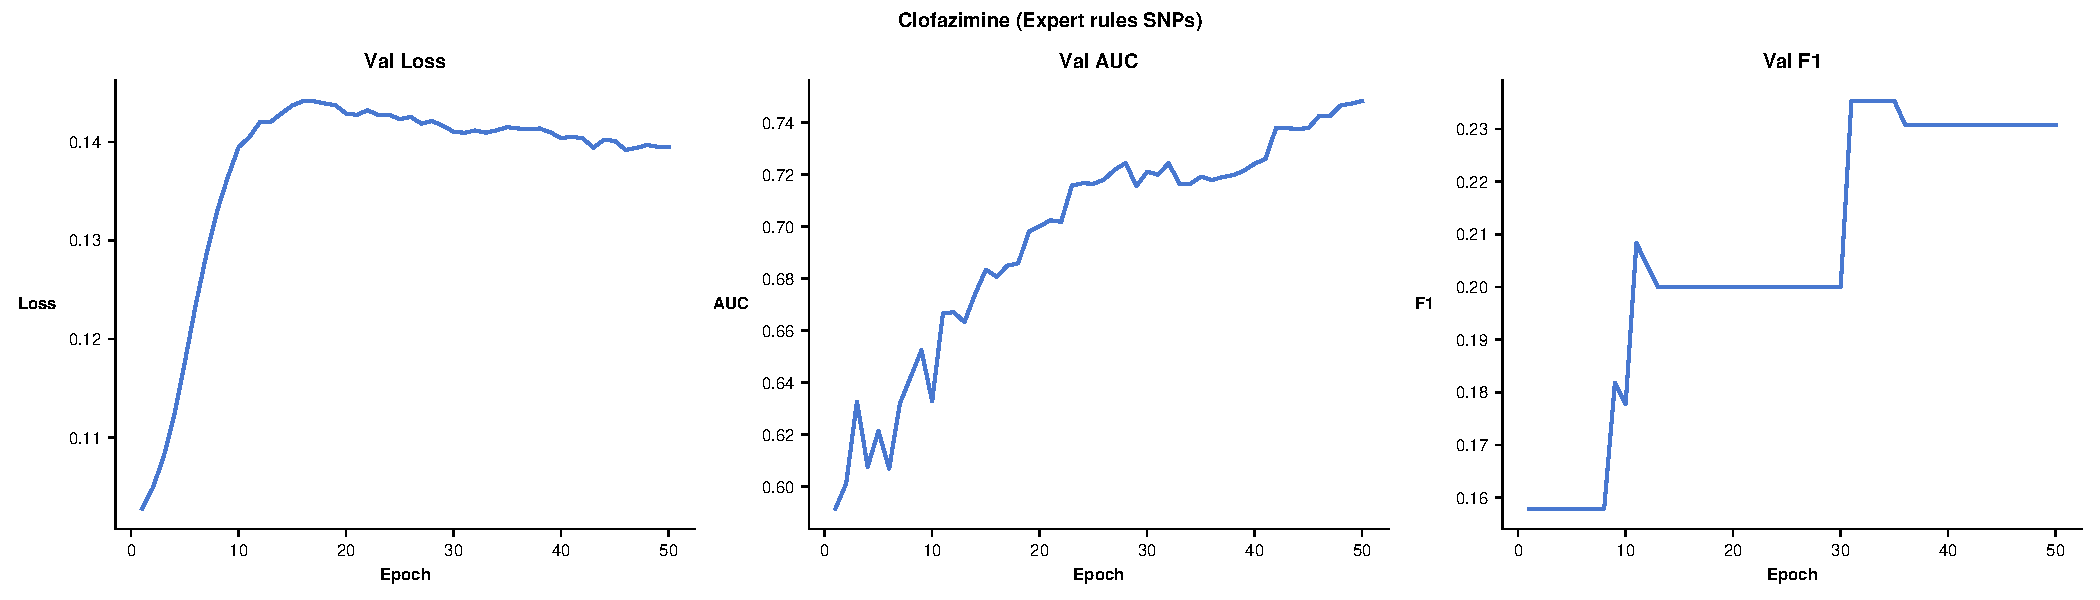
\includegraphics[width=\textwidth]{figures/expert_rules_clofazimine_learning_curves.pdf}
    \end{subfigure}
    \begin{subfigure}{\textwidth}
        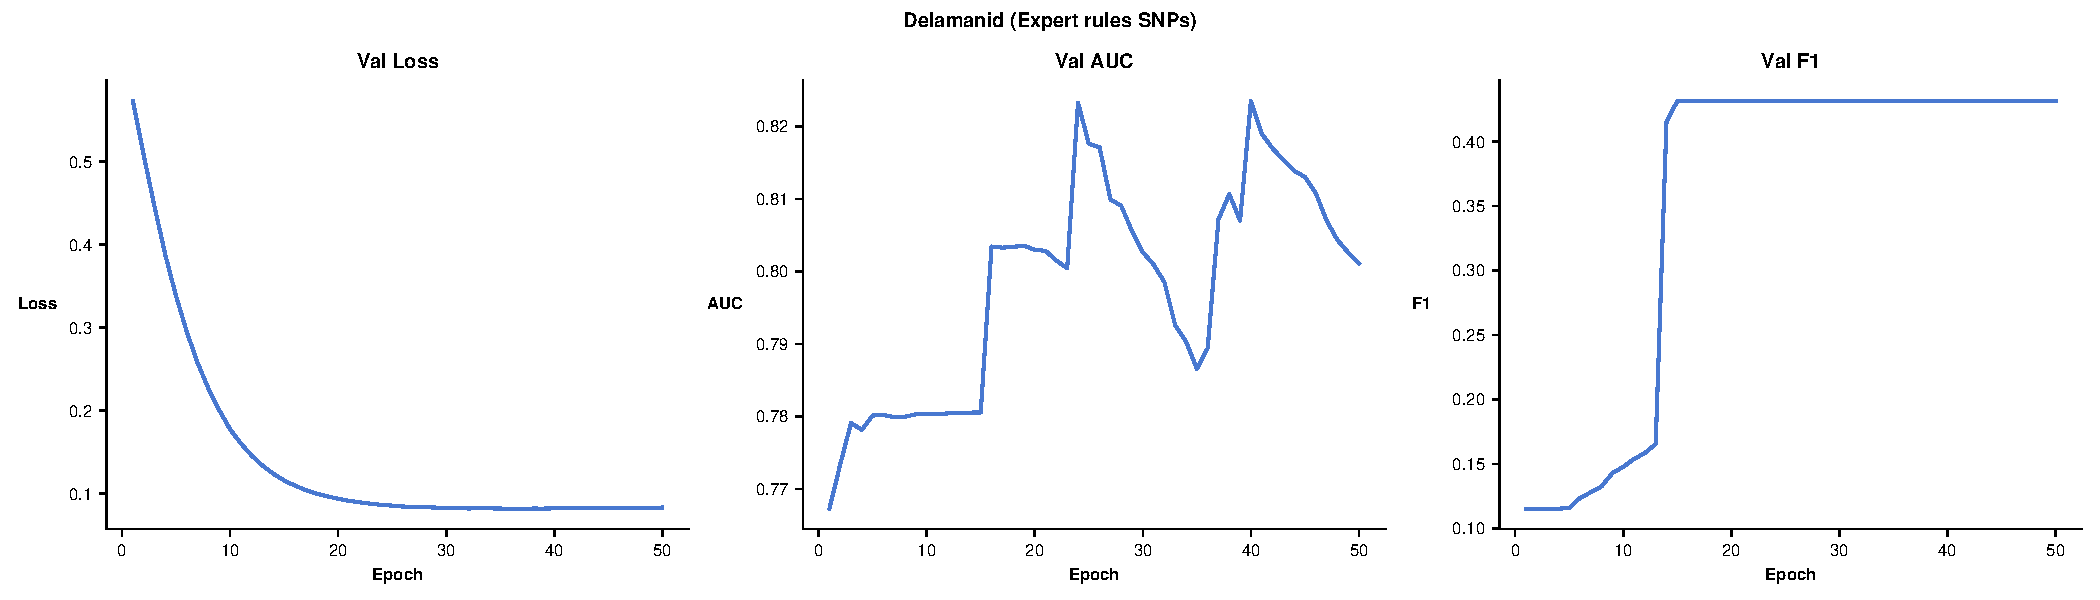
\includegraphics[width=\textwidth]{figures/expert_rules_delamanid_learning_curves.pdf}
    \end{subfigure}
    \begin{subfigure}{\textwidth}
        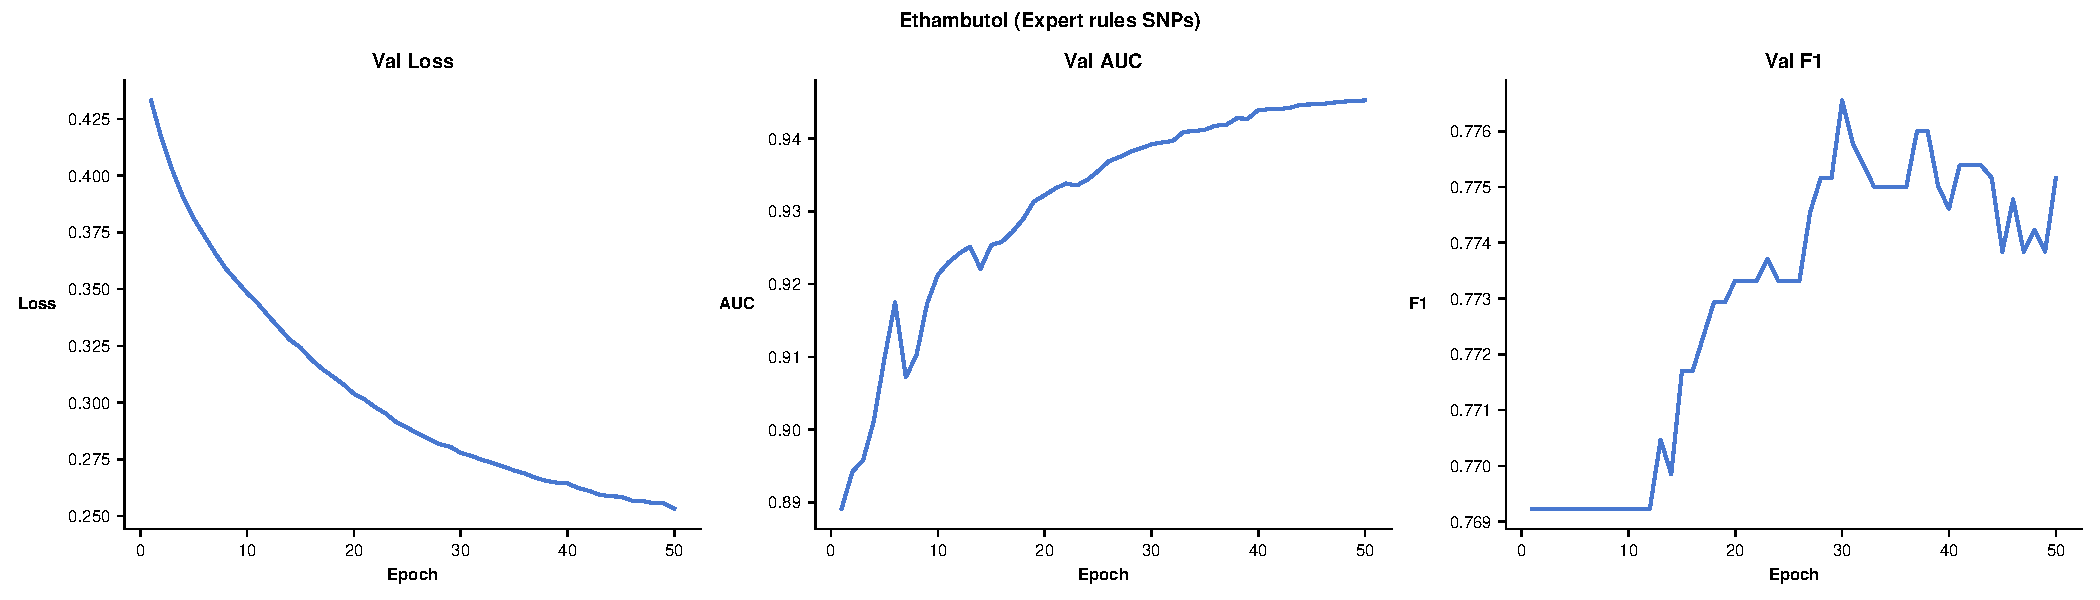
\includegraphics[width=\textwidth]{figures/expert_rules_ethambutol_learning_curves.pdf}
    \end{subfigure}
\end{figure}

\begin{figure}[H]
    \ContinuedFloat
    \centering
    \begin{subfigure}{\textwidth}
        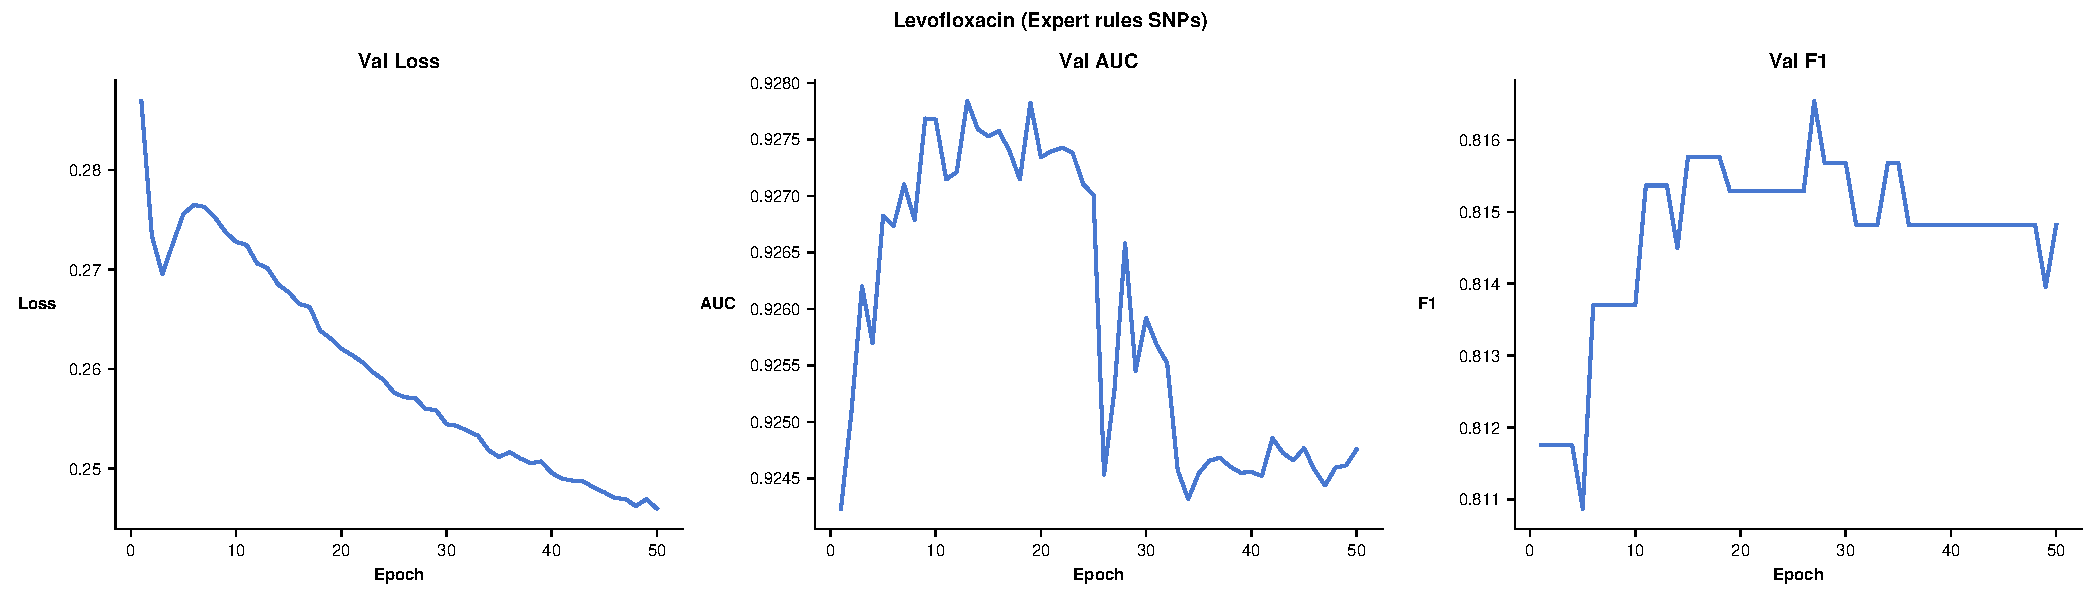
\includegraphics[width=\textwidth]{figures/expert_rules_levofloxacin_learning_curves.pdf}
    \end{subfigure}
    \begin{subfigure}{\textwidth}
        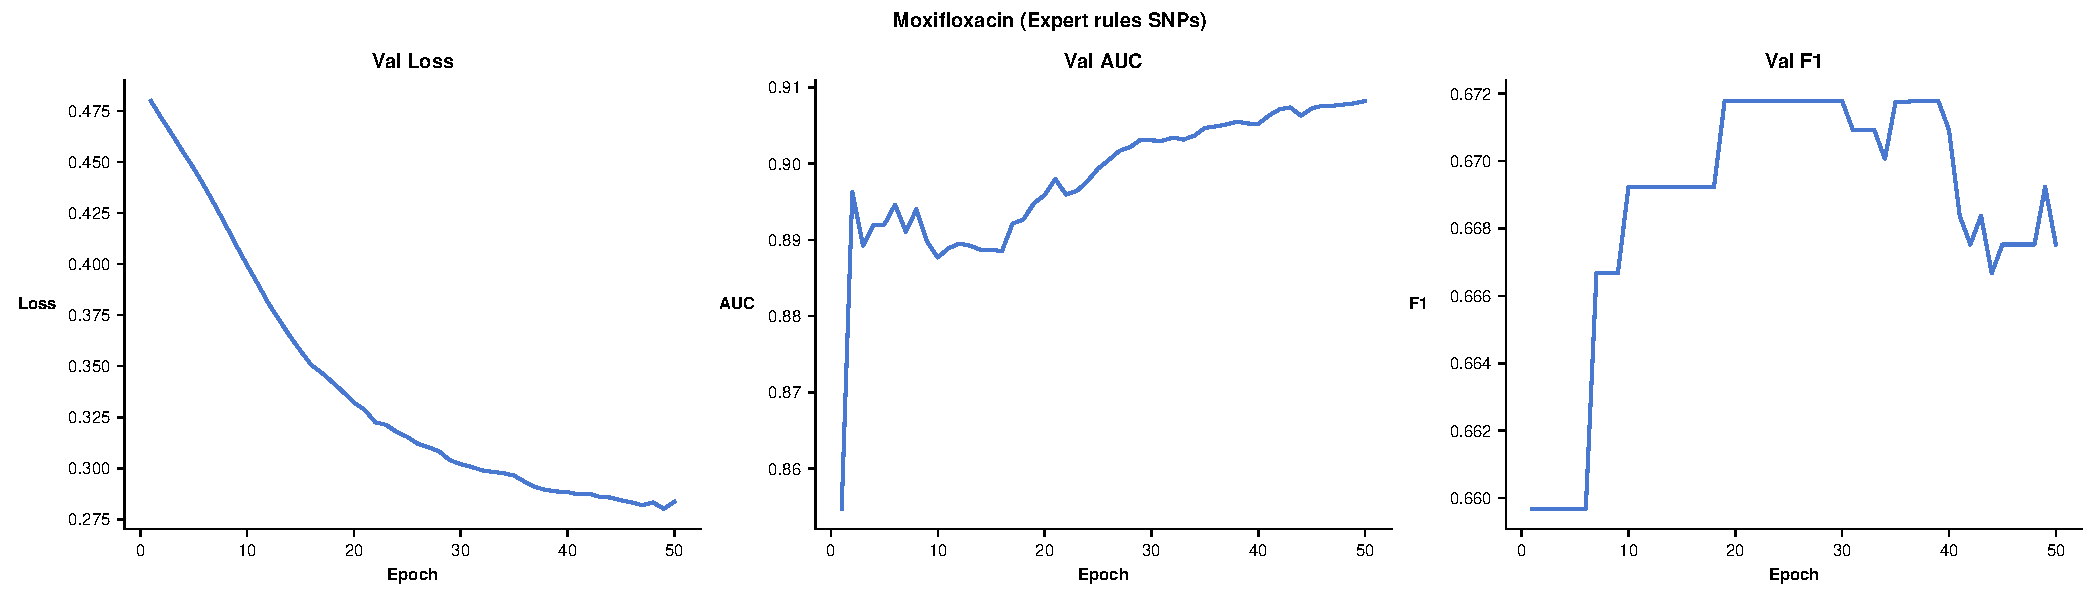
\includegraphics[width=\textwidth]{figures/expert_rules_moxifloxacin_learning_curves.pdf}
    \end{subfigure}
    \begin{subfigure}{\textwidth}
        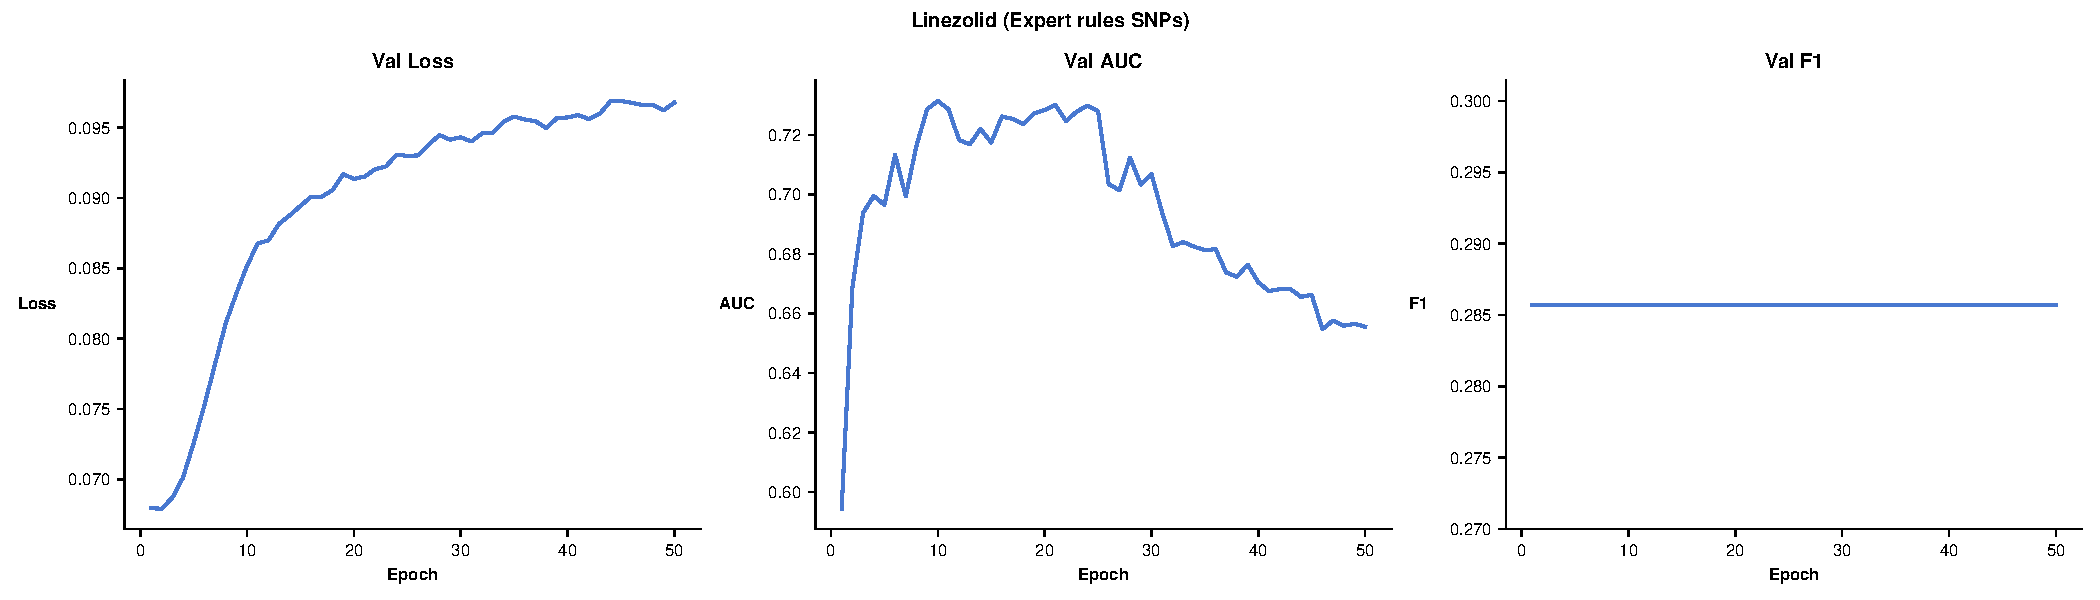
\includegraphics[width=\textwidth]{figures/expert_rules_linezolid_learning_curves.pdf}
    \end{subfigure}
    \caption{Model performance across all drugs}  % caption only on last block
    \label{fig:all_drugs}
\end{figure}
